\section{Written Questions}
\label{sec:written}

Write your solutions to the HW5 Written Questions in this template. You may either enter your solutions into the .tex file directly, or print out the pdf version and write your solutions by hand in the boxes provided.  When you have completed all of the written questions, you should upload your solutions to Gradescope in pdf format.
    
\subsection{Example Feed Forward and Backpropagation}
\label{sec:onelayertoy}

 \begin{figure}[h]
        \centering
        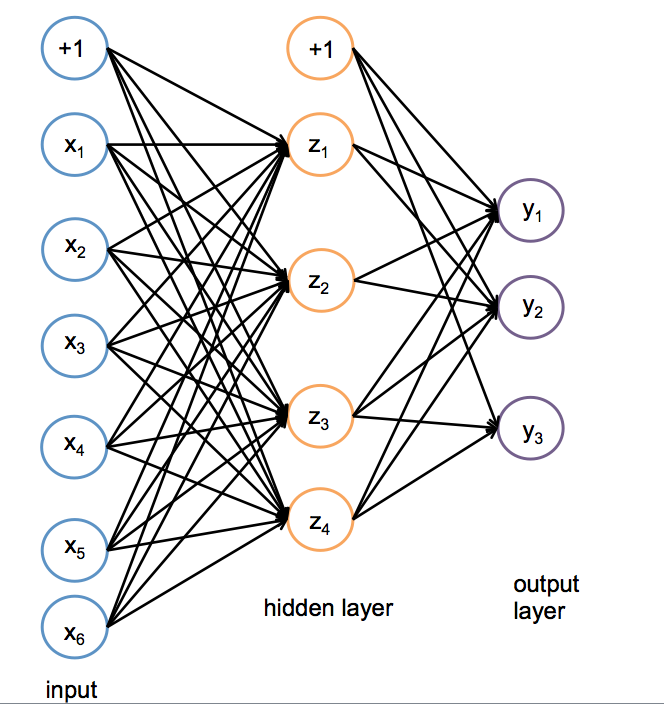
\includegraphics[scale=0.7]{oneHL6.png}
        \caption{A One Hidden Layer Neural Network}
        \label{fig:oneHL}
    \end{figure}


Consider the neural network with one hidden layer shown in Figure \ref{fig:oneHL}. The inputs have 6 features ($x_1,...,x_6$), the hidden layer has 4  nodes ($z_1,...,z_4$), and the output is a probability distribution $(y_1, y_2, y_3)$ over 3 classes . We also add a bias to the input, $x_0$, as well as to the hidden layer, $z_0$ and set them to 1.
$\boldsymbol{\alpha}$ is the matrix of weights from the inputs to the hidden layer and $\boldsymbol{\beta}$ is the matrix of weights from the hidden layer to the output layer. 
$\alpha_{j,i}$ represents the weight going \textit{to} the node $z_j$ in the hidden layer \textit{from} the node $x_i$ in the input layer (e.g. $\alpha_{1,2}$ is the weight from $x_2$ to $z_1$), and $\boldsymbol{\beta}$ is defined similarly. We will use a sigmoid activation function for the hidden layer and a softmax for the output layer.

Equivalently, we define each of the following. The input:

\begin{align}
\bold{x}=(x_1,x_2,x_3,x_4,x_5,x_6)
\end{align}

Linear combination at first (hidden) layer:
\begin{equation}
a_j= \alpha_0 + \sum_{i=1}^6 \alpha_{j,i}*x_i,\,\, \forall j \in \{1,\ldots,6\}
\end{equation}

Activation at first (hidden) layer:
\begin{align}
z_j &= \sigma(a_j) = \frac{1}{1+\exp(-a_j)},\,\, \forall j \in \{1,\ldots,6\}
\end{align}

Linear combination at second (output) layer:
\begin{equation}
b_k = \beta_0 + \sum_{j=1}^4 \beta_{k,j}*z_j,\,\, \forall k \in \{1,\ldots,3\}
\end{equation}

Activation at second (output) layer:
\begin{equation}
y_k = \frac{\exp(b_k)}{\sum\limits_{l=1}^3 \exp(b_l)},\,\, \forall k \in \{1,\ldots,3\}
\end{equation}

Note that the linear combination equations can be written equivalently as the product of the transpose of the weight matrix with the input vector. We can even fold in the bias term $\alpha_0$ by thinking of $x_0 = 1$, and fold in $\beta_0$ by thinking of $z_0 = 1$.

We will use cross entropy loss, $\ell(\hat{\yv},\yv)$. If $\yv$ represents our target output, which will be a one-hot vector representing the correct class, and $\hat{\yv}$ represents the output of the network, the loss is calculated by:
\begin{equation}
   % \ell(\hat{y},y)=\frac{1}{2}\sum\limits_{i=1}^3(y_i-\hat{y}_i)^2
   \ell(\hat{\yv},\yv) = - \sum_{i=1}^3 y_i \log(\hat{y}_i)
\end{equation}

When doing prediction, we will predict the $\argmax$ of the output layer. For example, if $\hat{y}_1=0.3$, $\hat{y}_2=0.2$, $\hat{y}_3=0.5$ we would predict class 3.

\begin{enumerate} 
\item \points{4}
     We initialize the weights as:
\begin{center}
$$\boldsymbol{\alpha}=
    \begin{bmatrix}
    1 & 2 & -3 & 0 & 1 & -3 \\
    3 & 1 & 2 & 1 & 0 & 2 \\
    2 & 2 & 2 & 2 & 2 & 1 \\
    1 & 0 & 2 & 1 & -2 & 2
    \end{bmatrix}$$
    
$$\boldsymbol{\beta}=
    \begin{bmatrix}
    1 & 2 & -2 & 1 \\
    1 & -1 & 1 & 2 \\
    3 & 1 & -1 & 1
    \end{bmatrix}
$$
\end{center}
    
And weights on the bias terms (${\alpha}_{j,0}$ and ${\beta}_{j,0})$ are initialized to 1.
    
    You are given a training example $x^{(1)}=(1,1,0,0,1,1)$ with label class 2, so $y^{(1)}=(0,1,0)$. Using the initial weights, run the feed forward of the network over this example (without rounding) and then answer the following questions. In your responses, round to four decimal places (if the answer is an integer you need not include trailing zeros). (Note: the superscript $(1)$ simply indicates that a value corresponds to using training example $x^{(1)}$)
    
    \begin{enumerate}
        \item What is $a^{(1)}_1$?
        
        (Please include one number rounded to the fourth decimal place, e.g. 0.1234)
    
        \begin{tcolorbox}[fit,height=1cm,blank, borderline={1pt}{-2pt},nobeforeafter]
        %Input your solution here.  Do not change any of the specifications of this solution box.
        \end{tcolorbox}
        
        \item What is $z^{(1)}_1$?
        
        (Please include one number rounded to the fourth decimal place, e.g. 0.1234)
    
        \begin{tcolorbox}[fit,height=1cm,blank, borderline={1pt}{-2pt},nobeforeafter]
        %Input your solution here.  Do not change any of the specifications of this solution box.
        \end{tcolorbox}
        
         \item What is $a^{(1)}_3$?
        
        (Please include one number rounded to the fourth decimal place, e.g. 0.1234)
    
        \begin{tcolorbox}[fit,height=1cm,blank, borderline={1pt}{-2pt},nobeforeafter]
        %Input your solution here.  Do not change any of the specifications of this solution box.
        \end{tcolorbox}
        
        \item What is $z^{(1)}_3$?
        
        (Please include one number rounded to the fourth decimal place, e.g. 0.1234)
    
        \begin{tcolorbox}[fit,height=1cm,blank, borderline={1pt}{-2pt},nobeforeafter]
        %Input your solution here.  Do not change any of the specifications of this solution box.
        \end{tcolorbox}
        
        \item What is $b^{(1)}_2$?
        
        (Please include one number rounded to the fourth decimal place, e.g. 0.1234)
        
        \begin{tcolorbox}[fit,height=1cm,blank, borderline={1pt}{-2pt},nobeforeafter]
        %Input your solution here.  Do not change any of the specifications of this solution box.
        \end{tcolorbox}
        
        \item What is $\hat{y}^{(1)}_2$?
        
        (Please include one number rounded to the fourth decimal place, e.g. 0.1234)
        
        \begin{tcolorbox}[fit,height=1cm,blank, borderline={1pt}{-2pt},nobeforeafter]
        %Input your solution here.  Do not change any of the specifications of this solution box.
        \end{tcolorbox}
        
        \item Which class would we predict on this example?
        
        \begin{tcolorbox}[fit,height=1cm,blank, borderline={1pt}{-2pt},nobeforeafter]
        %Input your solution here.  Do not change any of the specifications of this solution box.
        \end{tcolorbox}
        
        \item What is the total loss on this example?
        
        (Please include one number rounded to the fourth decimal place, e.g. 0.1234)
        
        \begin{tcolorbox}[fit,height=1cm,blank, borderline={1pt}{-2pt},nobeforeafter]
        %Input your solution here.  Do not change any of the specifications of this solution box.
        \end{tcolorbox}
        
    
    \end{enumerate}
    \clearpage
    \item \points{5} Now use the results of the previous question to run backpropagation over the network and update the weights. Use learning rate $\eta=1$. 
    
     Do your backpropagation calculations without rounding then answer the following questions, then in your responses, round to four decimal places
    
     \begin{enumerate}
        \item What is the updated value of ${\beta}_{2,1}$?
        
        (Please include one number rounded to the fourth decimal place, e.g. 0.1234)
        
        \begin{tcolorbox}[fit,height=1cm,blank, borderline={1pt}{-2pt},nobeforeafter]
        %Input your solution here.  Do not change any of the specifications of this solution box.
        \end{tcolorbox}
        
        \item What is the updated weight of the hidden layer bias term applied to $y_1$ (eg ${\beta}_{1,0}$)?
        
        (Please include one number rounded to the fourth decimal place, e.g. 0.1234)
        
        \begin{tcolorbox}[fit,height=1cm,blank, borderline={1pt}{-2pt},nobeforeafter]
        %Input your solution here.  Do not change any of the specifications of this solution box.
        \end{tcolorbox}
        
        \item What is the updated value of ${\alpha}_{3,4}$?
        
        (Please include one number rounded to the fourth decimal place, e.g. 0.1234)
        
        \begin{tcolorbox}[fit,height=1cm,blank, borderline={1pt}{-2pt},nobeforeafter]
        %Input your solution here.  Do not change any of the specifications of this solution box.
        \end{tcolorbox}
        
        \item What is the updated weight of the input layer bias term applied to $z_2$ (eg ${\alpha}_{2,0}$)?
        
        (Please include one number rounded to the fourth decimal place, e.g. 0.1234)
        
        \begin{tcolorbox}[fit,height=1cm,blank, borderline={1pt}{-2pt},nobeforeafter]
        %Input your solution here.  Do not change any of the specifications of this solution box.
        \end{tcolorbox}
        
        \item Once we've updated all of our weights if we ran feed forward over the same example again, which class would we predict?
        
        (Please include one number rounded to the fourth decimal place, e.g. 0.1234)
        
        \begin{tcolorbox}[fit,height=1cm,blank, borderline={1pt}{-2pt},nobeforeafter]
        %Input your solution here.  Do not change any of the specifications of this solution box.
        \end{tcolorbox}
        
    \end{enumerate}
   \item \points{1} Suppose you are now given a collection of training examples $\Dc = \{ (\xv^{(i)}, \yv^{(i)}) \}$. Explain in English why the cross-entropy loss averaged over these examples is exactly the same quantity as the negative average conditional log-likelihood of the data. 
   
   \begin{tcolorbox}[fit,height=3cm,blank, borderline={1pt}{-2pt},nobeforeafter]
        %Input your solution here.  Do not change any of the specifications of this solution box.
    \end{tcolorbox}
   
\end{enumerate}
%\clearpage
\subsection{Empirical Questions \points{10}}
\label{sec:interp}

The following questions should be completed after you work through the programming portion of this assignment

For these questions, use the large dataset.

Use the following values for the hyperparameters unless otherwise specified:

\begin{table}[H]
    \centering
    \begin{tabular}{|c|c|}
        \hline
        \textbf{Paramater} & \textbf{Value} \\
        \hline
        Number of Hidden Units & 50 \\
        \hline
        Weight Initialization & 0.1 \\
        \hline
        Learning Rate & 0.01 \\
        \hline
        
    \end{tabular}
    \caption{Default values of hyperparameters for experiments in Section \ref{sec:interp}.}
    \label{tab:params}
\end{table}
For the following questions, submit your solutions to Gradescope. Do {\bf not} include any visualization-related code when submitting to Autolab! Note: we expect it to take about {\bf 5 minutes} to train each of these networks.

\begin{enumerate}
\setcounter{enumi}{3}
\item \points{4}  %% hidden units
Train a single hidden layer neural network using the hyperparameters mentioned in Table \ref{tab:params}, except for the number of hidden units which should vary among 5, 20, 50, 100, and 200.  Run the optimization for 100 epochs each time.

Plot the average training cross-entropy (sum of the cross-entropy terms over the training dataset divided by the total number of training examples) on the y-axis vs number of hidden units on the x-axis. On the same figure, plot the average validation cross-entropy.

\begin{tcolorbox}[fit,height=11cm,blank, borderline={1pt}{-2pt},nobeforeafter]
        %Input your plot here.  Do not change any of the specifications of this solution box.
\end{tcolorbox}

\item \points{1} Examine and comment on the the plots of training error and validation error. What effect does changing the number of hidden units have?

\begin{tcolorbox}[fit,height=4cm,blank, borderline={1pt}{-2pt},nobeforeafter]
        %Input your comments here.  Do not change any of the specifications of this solution box.
        \end{tcolorbox}
        
%\clearpage        
        
\item \points{4} %%% different learning rates
Train a single hidden layer neural network using the hyperparameters mentioned in Table \ref{tab:params}, except for the learning rate which should vary among 0.1, 0.01, and 0.001. Run the optimization for 100 epochs each time.

Plot the average training cross-entropy on the y-axis vs the number of epochs on the x-axis for the mentioned learning rates. On the same figure, plot the average validation cross-entropy loss. You may make a separate figure for each learning rate.

\begin{tcolorbox}[fit,height=13.5cm,blank, borderline={1pt}{-2pt},nobeforeafter]
        %Input your plot(s) here.  Do not change any of the specifications of this solution box.
\end{tcolorbox}


\item \points{1} 
Examine and comment on the the plots of training and validation cross-entropy. How does adjusting the learning rate affect the convergence of cross-entropy of each dataset?

\begin{tcolorbox}[fit,height=4cm,blank, borderline={1pt}{-2pt},nobeforeafter]
        %Input your comments here.  Do not change any of the specifications of this solution box.
        \end{tcolorbox}

\item {\bf Collaboration Questions} After you have completed all other components of this assignment, report your answers to the collaboration policy questions detailed in the Academic Integrity Policies found \href{http://www.cs.cmu.edu/~mgormley/courses/10601-s18/about.html#7-academic-integrity-policies}{here}.
    \begin{enumerate*}
        \item Did you receive any help whatsoever from anyone in solving this assignment? Is so, include full details.
        \item Did you give any help whatsoever to anyone in solving this assignment? Is so, include full details?
        \item Did you find or come across code that implements any part of this assignment ? If so, include full details.
    \end{enumerate*}
    
    \begin{tcolorbox}[fit,height=3cm,blank, borderline={1pt}{-2pt},nobeforeafter]
    %Input your solution here.  Do not change any of the specifications of this solution box.
    \end{tcolorbox}

\end{enumerate}

